%%%%%%%%%%%%%%%%%%%%%%%%%%%%%%%%%%%%%%%%%%%%%%%%%%%%%%%%%%%%%%%%%%%%%%%%%%%%%%%%
%% MASTER'S THESIS                                                            %%
%%                                                                            %% 
%% Title (en): Multi-Agent Systems and Organizations                          %%
%% Title (cs): Multiagentní systémy a organizace                              %%
%%                                                                            %%
%% Author: Bc. Lukáš Kúdela                                                   %%
%% Supervisor: Prof. RNDr. Petr Štěpánek, DrSc.                               %%
%%                                                                            %%
%% Academic year: 2011/2012                                                   %%
%%%%%%%%%%%%%%%%%%%%%%%%%%%%%%%%%%%%%%%%%%%%%%%%%%%%%%%%%%%%%%%%%%%%%%%%%%%%%%%%

\chapter{Examples}

% Chapter abstract - Thespian4Jade examples
In this chapter, we will present three examples that demonstrate the use of the \textit{Thespian4Jade} module to model organizations in MASs.
The examples are ordered by the complexity of the MAS social structure---the first can be considered a toy problem, while the last one is a real-world problem.

% Examples - specification & manifestation
The MAS in each example is presented in two parts: specification and manifestation.
The specification part presents the model of the MAS and the manifestation part presents a potential run of the MAS.

% Specification - structure
In all examples, the MAS is modelled using three sub-models: a) organization and role model, b) protocol model and c) player model.

% Manifestation - structure
In all examples, the MAS runs in five stages: 1) role enactment, 2) role activation, 3) competence and responsibility invocation, 4) role deactivation and 5) role deactment.
The third stage is the problem-solving stage---a period of time during which the agents solve the problem itself by exercising their competences and fulfilling their responsibilities.
The other stages are infrastructure stages---time intervals during which agents organize themselves into organizations, enact/deact roles and activate/deactivate them.
For the first example, we will provide a detailed description of all five stages; for the second example, a brief description for all five stages will suffice; and for the third example, a brief description of the problem-solving stage will be sufficient.

% Assumptions
In all three examples, we assume
\begin{itemize}
	\item the concrete organization in which the agents want to participate already exists, and
	\item that the agents already know its AID\footnote{\textit{Agent ID}---an agent's address, in the format \textless{}agent-name\textgreater{}@\textless{}platform-name\textgreater{}.}.
\end{itemize}
Situations where the second assumption or even both assumptions do not hold lie outside the scope of this thesis (see Conclusion and Future Work).

% Complete agent interaction diagrams
The complete interaction diagrams\footnote{Diagrams showing interaction between agents in a MAS.} are too large to be reproduced here; they can be found on the companion CD-ROM. 

%%%%%%%%%%%%%%%%%%%%%%%%%%%%%%%%%%%%%%%%%%%%%%%%%%%%%%%%%%%%%%%%%%%%%%%%%%%%%%%%
%% MASTER'S THESIS                                                            %%
%%                                                                            %% 
%% Title (en): Multi-Agent Systems and Organizations                          %%
%% Title (cs): Multiagentní systémy a organizace                              %%
%%                                                                            %%
%% Author: Bc. Lukáš Kúdela                                                   %%
%% Supervisor: Prof. RNDr. Petr Štěpánek, DrSc.                               %%
%%                                                                            %%
%% Academic year: 2011/2012                                                   %%
%%%%%%%%%%%%%%%%%%%%%%%%%%%%%%%%%%%%%%%%%%%%%%%%%%%%%%%%%%%%%%%%%%%%%%%%%%%%%%%%
\section{Example 1: Function Invocation}

% Function invocation organization
This example demonstrates a simple organization -- the function invocation.
% Function invocation organization - purpose
The purpose of this organization is to facilitate remote function invocation by grouping two agents: one agent invokes a function and the other one executes it.
% Assumptions
In this example, an agent invokes the factorial function, but it should be obvious that any (computable) function could be invoked this way.

%%%%%%%%%%%%%%%%%%%%%%%%%%%%%%%%%%%%%%%%%%%%%%%%%%%%%%%%%%%%%%%%%%%%%%%%%%%%%%%%
\subsection*{Specification}

%%%%%%%%%%%%%%%%%%%%%%%%%%%%%%%%%%%%%%%%%%%%%%%%%%%%%%%%%%%%%%%%%%%%%%%%%%%%%%%%
\subsubsection*{Organization Part}

% 'Function invocation' organization type
The \textit{Invoke function} organization type (modelled by the \texttt{FunctionInvocation\_Organization} agent class) contains two roles -- \textit{Asker} and \textit{Answerer} -- and one protocol -- \textit{Invoke function}.
% 'function-invocation' organization
\textit{Invoke function} has one instance in the running MAS -- the \textit{invoke-function} organization (modelled by the \texttt{invokeFunction\_Organization} agent instance).

% 'Invoker' role
The \textit{Invoker} role (modelled by the \texttt{Invoker\_Role} class) can invoke (not compute) a function to be executed.
% 'Invoker' role - multiplicity, competences & responsibilities
The \textit{Invoker} role is a \textit{single} role.
It has one competence -- \textit{Invoke function} -- and no responsibilities.

% 'Invoke function' competence
The \textit{Invoke function} competence (modelled by the \texttt{InvokeFunction\_Competence} class) is a competence to invoke a function.
% 'Invoke function' competence - argument & result
It has one argument -- the function argument -- and one result -- the function value. 

% 'Executer' role
The \textit{Executer} role (modelled by the \texttt{Executer\_Role} class) can execute a function upon its invocation.
% 'Execute' role - multiplicity, competences & responsibilities
The \textit{Executer} role is a \textit{single} role.
It has no competences and one responsibility -- \textit{Execute function}.

% 'Execute function' responsibility
The \textit{Execute function} responsibility (modelled by the \texttt{ExecuteFunction\_Responsibility} class) is a responsibility to execute a function together for some argument.
% 'Execute function' responsibility - argument & result
It has one argument -- the function argument -- and one result -- the function value.

%%%%%%%%%%%%%%%%%%%%%%%%%%%%%%%%%%%%%%%%%%%%%%%%%%%%%%%%%%%%%%%%%%%%%%%%%%%%%%%%
\subsubsection*{Protocol Part}

% 'Invoke function' protocol
The \textit{Invoke function} protocol (modelled by the \texttt{InvokeFunctionProtocol} class) is a protocol by which an \textit{Invoker} (the initiator party, modelled by the \texttt{InvokeFunction\_InitiatorParty}) requests an \textit{Executor} (the responder party, modelled by the \texttt{InvokeFunction\_RespodnerParty}) to execute a function (the factorial function in this example).

% 'Invoke function request' message
The \textit{Invoke function request} message (modelled by the \texttt{InvokeFunctionRequestMessage} class) is a message sent by an \textit{Invoker} to an \textit{Executor} requesting the latter to execute a function for a particular argument.

% 'Invoke function reply' message
The \textit{Invoke function reply} message (modelled by the \texttt{InvokeFunctionReplyMessage} class) is a message sent by an \textit{Executer} to an \textit{Invoker} informing the latter about the value of the executed function.

\subsubsection*{Player Part}

% 'Blank' player type
The \textit{Blank} player type (modelled by the \texttt{Blank\_Player} agent class) is a player with no capabilities.
It has one instance in the running MAS -- \textit{player1}.
% 'player1' player
\textit{player1} (modelled by the \texttt{player1} agent instance) intends to enact the \textit{Invoker} role in the \textit{invoke-function} organization and to perform the role's \textit{Invoke function} competence -- to invoke a function to be executed by the player of the \textit{Executer} role.

% 'Factorial computer' player type
The \textit{Factorial computer} player type (modelled by the \texttt{FactorialComputer\_Player} agent class) is a player capable of computing the factorial function.
It has one instance in the running MAS -- \textit{player2}.
% 'player2' player
The intention of \textit{player2} (modelled by the \texttt{player2} agent instance) is to enact the \textit{Executer} role in the \textit{invoke-organization} organization and perform the role's \textit{Execute function} responsibility -- to execute the function invoked by the player of the \textit{Invoker} role.

%%%%%%%%%%%%%%%%%%%%%%%%%%%%%%%%%%%%%%%%%%%%%%%%%%%%%%%%%%%%%%%%%%%%%%%%%%%%%%%%
\subsection*{Manifestation}

%%%%%%%%%%%%%%%%%%%%%%%%%%%%%%%%%%%%%%%%%%%%%%%%%%%%%%%%%%%%%%%%%%%%%%%%%%%%%%%%
\subsubsection*{Stage 1: Role Enactment}

% Figure: Stage 1: Role enactment
\begin{figure}[H]
	\centering
	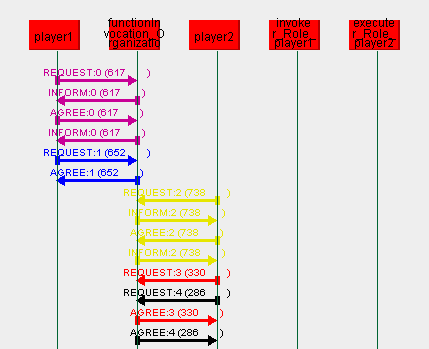
\includegraphics[width=0.8\textwidth]{images/examples/example1-stage1.png}
	\caption{Stage 1: Role enactment}
	\label{figure:example1-stage1}
\end{figure}

% Purple
The \textbf{purple} interaction scenario between \textit{player1} and the \textit{function-invocation} organization follows the \textit{Enact role} protocol.
\textit{player1} requests \textit{invoke-function} to enact the \textit{Invoker} role (1\textsuperscript{st} message) and is informed about the role's responsibilities (2\textsuperscript{nd} message) .
Since \textit{Invoker} has no responsibilities, \textit{player1} agrees that it can indeed enact the role (3\textsuperscript{rd} message).
\textit{invoke-organization} then creates the \textit{invoker-player1} position (modelled by the \texttt{invoker\_Role\_player1} agent instance) and informs \textit{player1} of its AID (4\textsuperscript{th} message).

% Blue
The \textbf{blue} interaction scenario between \textit{player1} and the \textit{function-invocation} organization follows the \textit{Subscribe to event} protocol.
\textit{player1} requests \textit{invoke-function} to subscribe to the \textit{Role activated} event (1\textsuperscript{st} message) and \textit{function-invocation} agrees (2\textsuperscript{nd} message).

% Yellow
The \textbf{yellow} interaction scenario between \textit{player2} and the \textit{invoke-function} organization follows the \textit{Enact role} protocol.
\textit{player2} requests \textit{invoke-function} to enact the \textit{Executer} role (1\textsuperscript{st}) and is informed about the role's responsibilities (2\textsuperscript{nd} message).
Since \textit{player2} can perform one \textit{Executer}'s responsibility -- the \textit{Execute function} responsibility -- it agrees that it can indeed enact the role (3\textsuperscript{rd} message).
\textit{invoke-function} then creates the \textit{executer-player2} position (modelled by the \texttt{executer\_Role\_player2} agent instance) and informs \textit{player2} of its AID (4\textsuperscript{th} message).

% Red
The \textbf{red} interaction scenario between t\textit{player2} and the \textit{function-invocation} organization follows the \textit{Subscribe to event} protocol.
\textit{player2} requests \textit{invoke-function} to subscribe to the \textit{Role activated} event (1\textsuperscript{st} message) and \textit{function-invocation} agrees (2\textsuperscript{nd} message).

% Black
The \textbf{black} interaction scenario between \textit{player2} and the \textit{function-invocation} organization follows the \textit{Subscribe to event} protocol.
\textit{player2} requests \textit{invoke-function} to subscribe to the \textit{Role deactivated} event (1\textsuperscript{st} message) and \textit{function-invocation} agrees (2\textsuperscript{nd} message).

%%%%%%%%%%%%%%%%%%%%%%%%%%%%%%%%%%%%%%%%%%%%%%%%%%%%%%%%%%%%%%%%%%%%%%%%%%%%%%%%
\subsubsection*{Stage 2: Role Activation}

% Figure: Stage 2: Role activation
\begin{figure}[H]
	\centering
	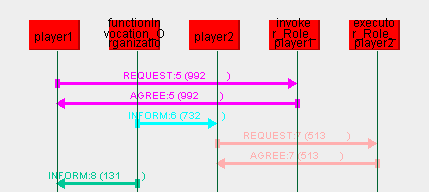
\includegraphics[width=0.8\textwidth]{images/examples/example1-stage2.png}
	\caption{Stage 2: Role activation}
	\label{figure:example1-stage2}
\end{figure}

% Magenta
The \textbf{magenta} interaction scenario between \textit{player1} and the \textit{invoker-player1} position follows the \textit{Activate role} protocol.
\textit{player1} requests \textit{invoker-player1} to activate the role (1\textsuperscript{st} message) and the position promptly agrees (2\textsuperscript{nd} message).

% Cyan
The \textbf{cyan} interaction scenario between the \textit{invoke-function} organization and \textit{player2} follows the \textit{Publish event} protocol.
\textit{invoke-organization} raises a \textit{Role activated} event (for the \textit{Invoker} role) and \textit{player2} handles it by activating its \textit{Executer} role (the \textbf{pink} interaction scenario).

% Pink
The \textbf{pink} interaction scenario between \textit{player2} and the \textit{executer-player2} position follows the \textit{Activate role} protocol.
\textit{player2} requests \textit{executer-player2} to activate the role (1\textsuperscript{st} message) and the position immediately agrees (2\textsuperscript{nd} message).

% Dark green
The \textbf{dark green} interaction scenario between the \textit{invoke-function} organization and \textit{player1} follows the \textit{Publish event} protocol.
\textit{invoke-organization} raises a \textit{Role activated} event (for the \textit{Executer} role) and \textit{player1} handles it by invoking the \textit{Invoke function} competence (the \textbf{light green} interaction scenario).

%%%%%%%%%%%%%%%%%%%%%%%%%%%%%%%%%%%%%%%%%%%%%%%%%%%%%%%%%%%%%%%%%%%%%%%%%%%%%%%%
\subsubsection*{Stage 3: Competence and Responsibility Invocation}

% Figure: Stage 3: Competence and responsibility invocation
\begin{figure}[H]
	\centering
	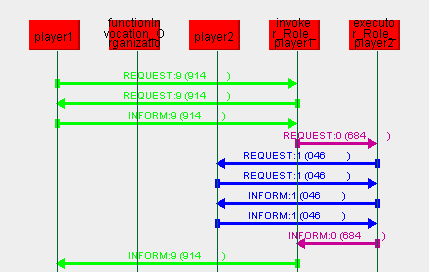
\includegraphics[width=0.8\textwidth]{images/examples/example1-stage3.png}
	\caption{Stage 3: Competence and responsibility invocation}
	\label{figure:example1-stage3}
\end{figure}

% Note - `Invoke competence' protocol vs. 'Invoke function' competence
In the following discussion, is is important to keep in mind that the \textit{Invoke competence} protocol is being used to invoke the \textit{Invoke function} competence.
Understanding the distinction between these two usages of the word `invoke' is a prerequisite to understanding the discussion of Stage 3.

% Light green
The \textbf{light green} interaction scenario between \textit{player1} and the \textit{invoker-player1} position follows the \textit{Invoke competence} protocol.
\textit{player1} requests \textit{invoker-player1} to invoke the \textit{Invoke function} competence (1\textsuperscript{st} message) and is in turn requested to provide the competence argument (2\textsuperscript{nd} message).
\textit{player1} then promptly informs \textit{invoker-player1} about the argument (3\textsuperscript{rd} message).
After \textit{invoker-player1} executes the competence (the \textbf{purple} interaction scenario), it informs \textit{player1} about its result (4\textsuperscript{th} message).

% Purple
The \textbf{purple} interaction scenario between the \textit{initiator-player1} and \textit{executer-player2} positions follows the \textit{Invoke function} protocol.
\textit{initiator-player1} requests \textit{executer-player2} to execute a particular function (factorial) for a particular argument (10, 1\textsuperscript{st} message).
\textit{executer-player2}, after invoking the \textit{Execute function} responsibility on its player (the \textbf{blue} interaction scenario), informs \textit{invoker-player1} about the function return value (3628800, 2\textsuperscript{nd} message).

% Blue
The \textbf{blue} interaction scenario between the \textit{executer-player2} position \textit{player2} follows the \textit{Invoke responsibility} protocol.
\textit{executer-player2} requests \textit{player2} to invoke the \textit{Execute function} responsibility (1\textsuperscript{st} message) and is in turn requested to provide the responsibility argument (2\textsuperscript{nd} message).
\textit{executer-player2} then immediately informs \textit{player2} about the argument (3\textsuperscript{rd} message).
After \textit{player2} executes the responsibility, it informs \textit{executer-player2} about its result (4\textsuperscript{th} message).

%%%%%%%%%%%%%%%%%%%%%%%%%%%%%%%%%%%%%%%%%%%%%%%%%%%%%%%%%%%%%%%%%%%%%%%%%%%%%%%%
\subsubsection*{Stage 4: Role Deactivation}

% Figure: Stage 4: Role deactivation
\begin{figure}[H]
	\centering
	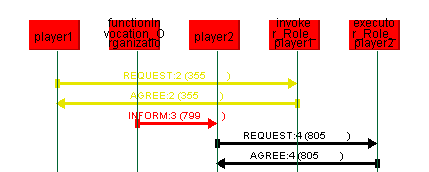
\includegraphics[width=0.8\textwidth]{images/examples/example1-stage4.png}
	\caption{Stage 4: Role deactivation}
	\label{figure:example1-stage4}
\end{figure}

% Yellow
The \textbf{yellow} interaction scenario between \textit{player1}  and the \textit{invoker-player1} position.
\textit{player1} requests \textit{invoker-player1} to deactivate the role (1\textsuperscript{st} message) and the position promptly agrees (2\textsuperscript{nd} message).

% Red
The \textbf{red} interaction scenario between the \textit{invoke-function} organization and \textit{player2} follows the \textit{Publish event} protocol.
\textit{invoke-organization} raises a \textit{Role deactivated} event (for the \textit{Invoker} role) and \textit{player2} handles it by deactivating its \textit{Executer} role (the \textbf{light green} interaction scenario).

% Black
The \textbf{black} interaction scenario between \textit{player2} and the \textit{executer-player2} position.
\textit{player2} requests \textit{executer-player2} to deactivate the role (1\textsuperscript{st} message) and the position immediately agrees (2\textsuperscript{nd} message).

%%%%%%%%%%%%%%%%%%%%%%%%%%%%%%%%%%%%%%%%%%%%%%%%%%%%%%%%%%%%%%%%%%%%%%%%%%%%%%%%
\subsubsection*{Stage 5: Role Deactment}

% Figure: Stage 5: Role deactment
\begin{figure}[H]
	\centering
	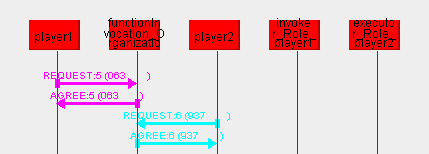
\includegraphics[width=0.8\textwidth]{images/examples/example1-stage5.png}
	\caption{Stage 5: Role deactment}
	\label{figure:example1-stage5}
\end{figure} 

% Magenta
The \textbf{magenta} interaction scenario between \textit{player1} and the \textit{invoke-function} organization.
\textit{player1} requests \textit{invoke-function} to deact the \textit{Invoker} role (1\textsuperscript{st} message) and the organization promptly agrees (2\textsuperscript{nd} message).

% Cyan
The \textbf{cyan} interaction scenario between \textit{player2} and the \textit{invoke-function} organizations.
\textit{player2} requests \textit{invoke-function} to deact the \textit{Executer} role (1\textsuperscript{st} message) and the organization immediately agrees (2\textsuperscript{nd} message).

%%%%%%%%%%%%%%%%%%%%%%%%%%%%%%%%%%%%%%%%%%%%%%%%%%%%%%%%%%%%%%%%%%%%%%%%%%%%%%%%
%% MASTER'S THESIS                                                            %%
%%                                                                            %% 
%% Title (en): Multi-Agent Systems and Organizations                          %%
%% Title (cs): Multiagentní systémy a organizace                              %%
%%                                                                            %%
%% Author: Bc. Lukáš Kúdela                                                   %%
%% Supervisor: Prof. RNDr. Petr Štěpánek, DrSc.                               %%
%%                                                                            %%
%% Academic year: 2011/2012                                                   %%
%%%%%%%%%%%%%%%%%%%%%%%%%%%%%%%%%%%%%%%%%%%%%%%%%%%%%%%%%%%%%%%%%%%%%%%%%%%%%%%%

\section{Example 2: Arithmetic Expression Evaluation}

% Section intro - 'Arithmetic expression evaluation' organziation
This example demonstrates a not-so-simple organization---\textit{arithmetic expression evaluation}.
% 'Arithmetic expression evaluation' - purpose
The purpose of this organization is to facilitate divide-and-conquer evaluation of arithmetic expressions by grouping five agents: one agent \textit{breaks the expression down} (the `divide' part) and the other four compute \textit{addition}, \textit{subtraction}, \textit{multiplication} and \textit{integral division} (the `conquer' part), each agent computing one arithmetic operation.
The reason the organization is formed in the first place is because the agent breaking the expression down is not capable of computing any arithmetic operation itself.
% Assumptions - simple arithmetic expression
In this example, agents evaluate simple arithmetic expressions---consisting of natural numbers, four basic arithmetic operations (addition, subtraction, multiplication and integral division) and parentheses. However, it should be apparent that any arithmetic expressions could be evaluated this way.

%%%%%%%%%%%%%%%%%%%%%%%%%%%%%%%%%%%%%%%%%%%%%%%%%%%%%%%%%%%%%%%%%%%%%%%%%%%%%%%%
\subsection*{Specification}

%%%%%%%%%%%%%%%%%%%%%%%%%%%%%%%%%%%%%%%%%%%%%%%%%%%%%%%%%%%%%%%%%%%%%%%%%%%%%%%%
\subsubsection*{Organization Part}

% 'Expression evaluation' organizaiton type
The \textit{Expression evaluation} organization type (modelled by the \texttt{ExpressionEvaluation\_Organization} agent class) contains five roles---\textit{Evaluator}, \textit{Adder}, \textit{Subtractor}, \textit{Multiplier} and \textit{Divider}---and two protocols---\textit{Evaluate expression} and \textit{Evaluate binary operation}.
% 'expression-evaluation' organization
\textit{Expression evaluation} has one instance in the running MAS: the \textit{expression-evaluation} organization (modelled by the \texttt{expressionEvaluation\_Organization} agent instance).

% 'Evaluator' role
The \textit{Evaluator} role (modelled by the \texttt{Evaluator\_Role} agent class) can evaluate a simple arithmetic expression.
% 'Evaluator' role - multiplicity, competences & responsibilities
The \textit{Evaluator} role is a \textit{multiple} role\footnote{However, only one agent plays the \textit{Evaluator} role in our example.}.
It has one competence---\textit{Evaluate}---and no responsibilities.

% 'Evaluate' competence
The \textit{Evaluate} competence (modelled by the \texttt{Evaluate\_Competence} class) is a competence to evaluate a simple arithmetic expression.
% 'Evaluate' competence - argument & result
It has one argument---an expression (a string)---and one result---the value of this expression (an integer).

% 'Adder' role
The \textit{Adder} role (modelled by the \texttt{Adder\_Role} agent class) can perform addition of two simple arithmetic expressions.
% 'Adder' role - multiplicity, competences & responsibilities
% TODO Consider making the binary operator roles multiple.
The \textit{Adder} role is a \textit{multiple} role\footnote{However, only one agent plays the \textit{Adder} role in our example.}.
It has no competences and one responsibility---\textit{Add}.

% 'Add' responsibility
The \textit{Add} responsibility (modelled by the \texttt{Add\_Responsibility} class) is a responsibility to perform addition of two integers.
% 'Add' responsibility - argument & result
It has two arguments---a pair of addends---and one result---their sum.

% 'Subtractor' role
The \textit{Subtractor} role (modelled by the \texttt{Subtractor\_Role} agent class) can perform subtraction of two simple arithmetic expressions.
% 'Subtractor' role - multiplicity, competences & responsibilities
The \textit{Subtractor} role is a \textit{multiple} role\footnote{However, only one agent plays the \textit{Subtractor} role in our example.}.
It has no competences and one responsibility---\textit{Subtract}.

% 'Subtract' responsibility
The \textit{Subtract} responsibility (modelled by the \texttt{Subtract\_Responsibility} class) is a responsibility to perform subtraction of two integers.
% 'Subtract' responsibility - argument & result
It has two arguments---a minuend and a subtrahend---and one result---their difference.

% 'Multiplier' role
The \textit{Multiplier} role (modelled by the \texttt{Multiplier\_Role} agent class) can perform multiplication of two simple arithmetic expressions.
% 'Multiplier' role - multiplicity, competences & responsibilities
The \textit{Multiplier} role is a \textit{multiple} role\footnote{However, only one agent plays the \textit{Multiplier} role in our example.}.
It has no competences and one responsibility---\textit{Multiply}.

% 'Multiply' responsibility
The \textit{Multiply} responsibility (modelled by the \texttt{Multiply\_Responsibility} class) is a responsibility to perform multiplication of two integers.
% 'Multiply' responsibility - argument & result
It has two arguments---a pair of factors---and one result---their product.

% 'Divider' role
The \textit{Divider} role (modelled by the \texttt{Divider\_Role} agent class) can perform division of two simple arithmetic expressions.
% 'Divider' role - multiplicity, competences & responsibilities
The \textit{Divider} role is a \textit{multiple} role\footnote{However, only one agent plays the \textit{Divider} role in our example.}.
It has no competences and one responsibility---\textit{Divide}.

% 'Divide' responsibility
The \textit{Divide} responsibility (modelled by the \texttt{Divide\_Responsibility} class) is a responsibility to perform integral division of two integers.
% 'Multiply' responsibility - argument & result
It has two arguments---a dividend and a divisor---and one result---their quotient.

% 'Binary operator' role
In the following, we will use the \textit{Binary operator} abstract role to refer to refer to the \textit{Adder}, \textit{Subtractor}, \textit{Multiplier} or \textit{Divisor} role where it is not necessary to distinguish between them.

%%%%%%%%%%%%%%%%%%%%%%%%%%%%%%%%%%%%%%%%%%%%%%%%%%%%%%%%%%%%%%%%%%%%%%%%%%%%%%%%
\subsubsection*{Protocol Part}

% 'Evaluate expresion' protocol
The \textit{Evaluate expression} protocol (modelled by the \texttt{EvaluateExpressionProtocol} class) is a protocol by which a \textit{Binary operator} (the initiator party, modelled by the \texttt{EvaluateExpression\_InitiatorParty}) requests an \textit{Evaluator} (the responder party, modelled by the \texttt{EvaluateExpression\_ResponderParty}) to evaluate an expression.

% 'Evaluate expression request' message
The \textit{Evaluate expression request} message (modelled by the \texttt{EvaluateExpressionRequestMessage} class) is a message sent by a \textit{Binary operator} to an \textit{Evaluator} requesting the latter to evaluate an expression.

% 'Evalaute expression reply' message
The \textit{Evaluate expression reply} message (modelled by the \texttt{EvaluateExpressionReplyMessage} class) is a message sent by an \textit{Evaluator} to a \textit{Binary operator} informing the latter about the value of the evaluated expression.

% 'Evaluate binary operation' protocol
The \textit{Evaluate binary operation} protocol (modelled by the \texttt{EvaluateBinaryOperationProtocol} class) is a protocol by which an \textit{Evaluator} (the initiator party, modelled by the \texttt{EvaluateBinaryOperation\_InitiatorParty}) requests a \textit{Binary operator} (the responder party, modelled by the \texttt{EvaluateBinaryOperation\_ResponderParty}) to evaluate a binary operation.

% 'Evalaute binary operation request' message
The \textit{Evaluate binary operation request} message (modelled by the \texttt{EvaluateBinaryOperationReqestMessage} class) is a message sent by a \textit{Evaluator} to a \textit{Binary Operator} requesting the latter to evaluate a binary operation between two operand expressions.

% 'Evaluate binary operation reply' message
The \textit{Evaluate binary operation reply} message (modelled by the \texttt{EvaluateBinaryOperationReplyMessage} class) is a message sent by a \textit{Binary operator} to an \textit{Evaluator} informing the latter about the value of the evaluated binary operation.

%%%%%%%%%%%%%%%%%%%%%%%%%%%%%%%%%%%%%%%%%%%%%%%%%%%%%%%%%%%%%%%%%%%%%%%%%%%%%%%%
\subsubsection*{Player Part}

% 'Blank' player type
The \textit{Blank} player type (modelled by the \texttt{Blank\_Player} agent class) is a player with no capabilities.
It has one instance in the running MAS: \textit{player1}.
% 'player1' player
\textit{player1} (modelled by the \texttt{player1} agent instance) intends to enact the \textit{Evaluator} role in the \textit{expression-evaluation} organization and to exercise the role's \textit{Evaluate} competence---to have an expression evaluated by the players of the \textit{Binary operator} roles.

% 'Addition computer' player type
The \textit{Addition computer} player type (modelled by the \texttt{AdditionComputer\_Player} agent class) is a player capable of computing the addition operation.
It has one instance in the running MAS: \textit{player2}.
% 'player2' player
\textit{player2} (modelled by the \texttt{player2} agent instance) intends to enact the \textit{Adder} role in the \textit{expression-evaluation} organization and fulfil the role's \textit{Add} responsibility---to compute addition during the evaluation of the expression from the player of the \textit{Evaluator} role.

% 'Subtraction computer' player type
The \textit{Subtraction computer} player type (modelled by the \texttt{SubtractionComputer\_Player} agent class) is a player capable of computing the subtraction operation.
It has one instance in the running MAS: \textit{player3}.
% 'player3' player
The intention of \textit{player3} (modelled by the \texttt{player3} agent instance) is to enact the \textit{Subtractor} role in the \textbf{expression-evaluation} organization and perform the role's \textit{Subtract} responsibility---to compute subtraction during the evaluation of the expression from the player of the  \textit{Evaluator} role.

% 'Multiplication computer' player type
The \textit{Multiplication computer} player type (modelled by the \texttt{MultiplicationComputer\_Player} agent class) is a player capable of computing the multiplication operation.
It has one instance in the running MAS: \textit{player4}.
% 'player4' player
\textit{player4} (modelled by the \texttt{player4} agent instance) intends to enact the \textit{Multiplier} role in the \textit{expression-evaluation} organization and fulfil the role's \textit{Multiply} responsibility---to compute multiplication during the evaluation of the expression from the player of the \textit{Evaluator} role.

% 'Division computer' player type
The \textit{Division computer} player type (modelled by the \texttt{DivisionComputer\_Player} agent class) is a player capable of computing the division operation.
It has one instance in the running MAS: \textit{player5}.
% 'player5' player
The intention of \textit{player5} (modelled by the \texttt{player5} agent instance) is to enact the \textit{Divisor} role in the \textit{expression-evaluation} organization and fulfil the role's \textit{Divide} responsibility---to compute division during the evaluation of the expression from the player of the \textit{Evaluator} role.

%%%%%%%%%%%%%%%%%%%%%%%%%%%%%%%%%%%%%%%%%%%%%%%%%%%%%%%%%%%%%%%%%%%%%%%%%%%%%%%%
\subsection*{Manifestation}

%%%%%%%%%%%%%%%%%%%%%%%%%%%%%%%%%%%%%%%%%%%%%%%%%%%%%%%%%%%%%%%%%%%%%%%%%%%%%%%%
\subsubsection*{Stage 1: Role Enactment}

% Figure: Stage 1: Role enactment
\begin{figure}[H]
	\centering
	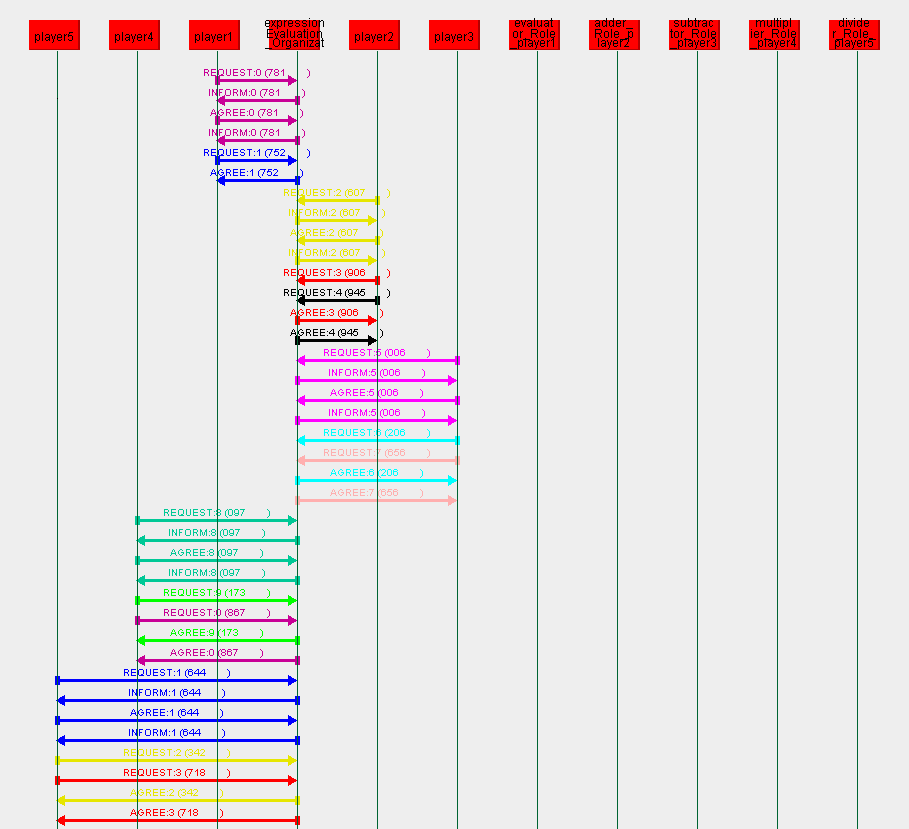
\includegraphics[width=\textwidth]{images/examples/example2-stage1.png}
	\caption{Stage 1: Role enactment}
	\label{figure:example2-stage1}
\end{figure}

% First purple
In the {\color{purple}{\textbf{first purple}}} interaction scenario, \textit{player1} enacts the \textit{Evaluator} role, resulting in the creation of the \textit{evaluator-player1} position.
% First blue
In the {\color{blue}{\textbf{first blue}}} interaction scenario, \textit{player1} subscribes to the \textit{Activate role} event.

% First yellow
In the {\color{yellow}{\textbf{first yellow}}} interaction scenario, \textit{player2} enacts the \textit{Adder} role, resulting in the creation of the \textit{adder-player2} position.
% First red & Black
In the {\color{red}{\textbf{first red}}} and {\color{black}{\textbf{black}}} interaction scenarios, \textit{player2} subscribes to the \textit{Activate role} and \textit{Deactivate role} events respectively.

% Magenta
In the {\color{magenta}{\textbf{magenta}}} interaction scenario, \textit{player3} enacts the \textit{Subtractor} role, resulting in the creation of the \textit{subtractor-player3} position.
% Cyan & Pink
In the {\color{cyan}{\textbf{cyan}}} and {\color{pink}{\textbf{pink}}} interaction scenarios, \textit{player3} subscribes to the \textit{Activate role} and \textit{Deactivate role} events respectively.

% Teal
In the {\color{teal}{\textbf{teal}}} interaction scenario, \textit{player4} enacts the \textit{Multiplier} role, resulting in the creation of the \textit{multiplier-player4} position.
% Green & Second purple
In the {\color{green}{\textbf{green}}} and {\color{purple}{\textbf{second purple}}} interaction scenarios, \textit{player4} subscribes to the \textit{Activate role} and \textit{Deactivate role} events respectively.

% Second blue
In the {\color{blue}{\textbf{second blue}}} interaction scenario, \textit{player5} enacts the \textit{Divider} role, resulting in the creation of the \textit{divider-player5} position.
% Second yellow & Second red
In the {\color{yellow}{\textbf{second yellow}}} and {\color{red}{\textbf{second red}}} interaction scenarios, \textit{player5} subscribes to the \textit{Activate role} and \textit{Deactivate role} events respectively.

%%%%%%%%%%%%%%%%%%%%%%%%%%%%%%%%%%%%%%%%%%%%%%%%%%%%%%%%%%%%%%%%%%%%%%%%%%%%%%%%
\subsubsection*{Stage 2: Role Activation}

% Figure: Stage 2: Role activation
\begin{figure}[H]
	\centering
	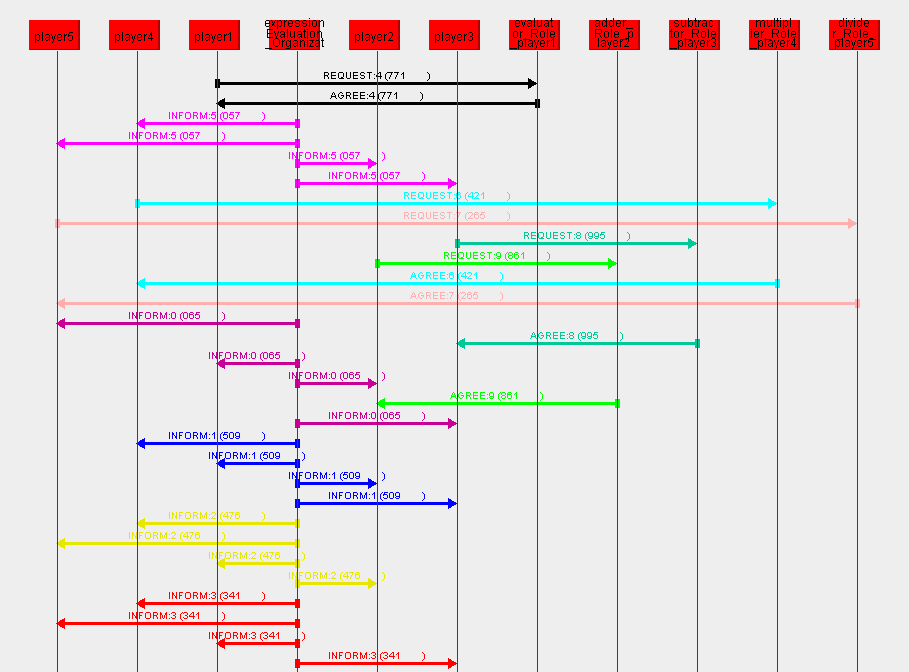
\includegraphics[width=\textwidth]{images/examples/example2-stage2.png}
	\caption{Stage 2: Role activation}
	\label{figure:example2-stage2}
\end{figure}

% Black
In the {\color{black}{\textbf{black}}} interaction scenario, \textit{player1} activates its \textit{Evaluator} role.
% Magenta
In the {\color{magenta}{\textbf{magenta}}} interaction scenario, the \textit{expression-evaluation} organization publishes the \textit{Role activated} event (for the \textit{Eveluator} role).
\textit{player2} reacts by activating its \textit{Adder} role (the {\color{green}{\textbf{green}}} interaction scenario), \textit{player3} by activating its \textit{Subtractor} role (the {\color{teal}{\textbf{teal}}} interaction scenario), \textit{player4} by activating its \textit{Multiplier} role (the {\color{cyan}{\textbf{cyan}}} interaction scenario) and \textit{player5} by activating its \textit{Divider} role (the {\color{pink}{\textbf{pink}}} interaction scenario).

% Green
In the {\color{green}{\textbf{green}}} interaction scenario, \textit{player2} activates its \textit{Adder} role.
% Red
In the {\color{red}{\textbf{red}}} interaction scenario, the \textit{expression-evaluation} organization publishes the \textit{Role activated} event (for the \textit{Adder} role).

% Teal
In the {\color{teal}{\textbf{teal}}} interaction scenario, \textit{player3} activates its \textit{Subtractor} role.
% Yellow
In the {\color{yellow}{\textbf{yellow}}} interaction scenario, the \textit{expression-evaluation} organization publishes the \textit{Role activated} event (for the \textit{Subtractor} role).

% Cyan
In the {\color{cyan}{\textbf{cyan}}} interaction scenario, \textit{player4} activates its \textit{Multiplier} role.
% Purple
In the {\color{purple}{\textbf{purple}}} interaction scenario, the \textit{expression-evaluation} organization publishes the \textit{Role activated} event (for the \textit{Multiplier} role).

% Pink
In the {\color{pink}{\textbf{pink}}} interaction scenario, \textit{player5} activates its \textit{Divider} role.
% Blue
In the {\color{blue}{\textbf{blue}}} interaction scenario, the \textit{expression-evaluation} organization publishes the \textit{Role activated} event (for the \textit{Divider} role).

% Event originator not notified
Note that that in all role activation scenarios, the player activating a role is not notified about the resulting \textit{Role activated} event, although it is subscribed to it; there is no need to notify the player causing the event in the first place.

%%%%%%%%%%%%%%%%%%%%%%%%%%%%%%%%%%%%%%%%%%%%%%%%%%%%%%%%%%%%%%%%%%%%%%%%%%%%%%%%
\subsubsection*{Stage 3: Competence and Responsibility Invocation}

% Figure: Stage 3: Competence and responsiility invocation
\begin{figure}[H]
	\centering
	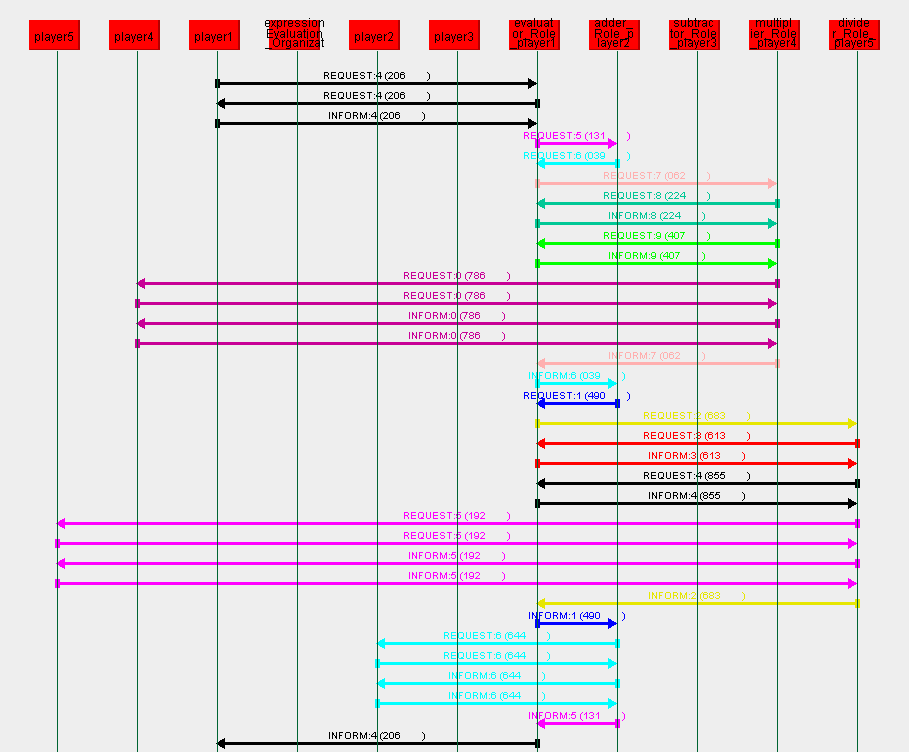
\includegraphics[width=\textwidth]{images/examples/example2-stage3.png}
	\caption{Stage 3: Competence and responsibility invocation}
	\label{figure:example2-stage3}
\end{figure}

The \textit{Evaluate expression} competence is invoked by \textit{player1} on its \textit{Evaluator} role and is carried out in a divide-and-conquer fashion by an \textit{Evaluator}, an \textit{Adder}, a \textit{Multiplier} and a \textit{Divider} by collaborating with one another and invoking responsibilities on their respective players.
In this example the arithmetic expression to be evaluated is $(1\cdot2)+(4/2)$.

% Evaluator: "(1*2)+(4/2)"
In the {\color{black}{\textbf{first black}}} interaction scenario, the \textit{evaluator-player1} position is requested by \textit{player1} to invoke the \textit{Evaluate} competence for the expression $(1\cdot2)+(4/2)$.
First, it parses the expression, finds the operation to be applied last---addition---and splits the expression into two sub-expressions to be added.
Next, it requests \textit{adder-player2} to evaluate their sum (the {\color{magenta}{\textbf{first magenta}}} interaction scenario).
Finally, it reports the value (4) to \textit{player1}.

% Adder: "(1*2)", "(4/2)"
In the {\color{magenta}{\textbf{first magenta}}} interaction scenario, the \textit{adder-player2} position is requested to evaluate the sum of the expressions $(1\cdot2)$ and $(4/2)$.
First, it requests \textit{evaluator-player1} to evaluate both expressions (the {\color{cyan}{\textbf{first cyan}}} and {\color{blue}{\textbf{blue}}} interaction scenarios).
Next, it invokes the \textit{Add} responsibility on \textit{player2} to calculate the sum of their values (the {\color{cyan}{\textbf{second cyan}}} interaction scenario).
Finally, it reports the sum (4) to \textit{evaluator-player1} (the original {\color{magenta}{\textbf{first magenta}}} interaction scenario).

% Evaluator: "(1*2)"
In the {\color{cyan}{\textbf{first cyan}}} interaction scenario, the \textit{evaluator-player1} position is requested to evaluate the expression $(1\cdot2)$.
First, it parses the expression, finds the last-to-be-applied operation---multiplication---and splits the expression into two sub-expressions to be multiplied.
Next, it requests \textit{multiplier-player4} to evaluate their product (the {\color{pink}{\textbf{pink}}} interaction scenario).
Finally, it reports the value (2) to \textit{adder-player2}.

% Multiplier: "1", "2"
In the {\color{pink}{\textbf{pink}}} interaction scenario, the \textit{multiplier-player4} position is requested to evaluate the product of the expressions $1$ and $2$.
First, it requests \textit{evaluator-player1} to evaluate both expressions (the {\color{teal}{\textbf{teal}}} and {\color{green}{\textbf{green}}} interaction scenarios).
Next, it invokes the \textit{Multiply} responsibility on \textit{player4} to calculate the product of their values (the {\color{purple}{\textbf{purple}}} interaction scenario).
Finally, it reports the product (2) to \textit{evaluator-player1} (the original {\color{pink}{\textbf{pink}}} interaction scenario).

% Evaluator: "1"
In {\color{teal}{\textbf{teal}}} interaction scenario, the \textit{evaluator-player1} is requested to evaluate the expression $1$.
It parses the expression, finds out it is a number (bottom case) and reports the value (1) to \textit{multiplier-player4}.

% Evaluator: "2"
In {\color{green}{\textbf{green}}} interaction scenario, the \textit{evaluator-player1} is requested to evaluate the expression $2$.
It parses the expression, finds out it is a number (bottom case) and reports the value (2) to \textit{multiplier-player4}.

% Evaluator: "(4/2)"
In the {\color{blue}{\textbf{blue}}} interaction scenario, the \textit{evaluator-player1} is requested to evaluate the expression $(4/2)$.
First, it parses the expression, finds the last-to-be-applied operation---division---and splits the expression into two sub-expressions to be divided.
Next, it requests \textit{divider-player5} to evaluate their product (the {\color{yellow}{\textbf{yellow}}} interaction scenario).
Finally, it reports the value (2) to \textit{adder-player2}.

% Divider: "4", "2"
In the {\color{yellow}{\textbf{yellow}}} interaction scenario, the \textit{divider-player5} position is requested to evaluate the quotient of the expressions $4$ and $2$.
First, it requests \textit{evaluator-player1} to evaluate both expressions (the {\color{red}{\textbf{red}}} and {\color{black}{\textbf{black}}} interaction scenarios).
Next, it invokes the \textit{Divide} responsibility on \textit{player5} to calculate the quotient of their values (the {\color{magenta}{\textbf{second magenta}}} interaction scenario).
Finally, it reports the quotient (2) to \textit{evaluator-player1} (the original {\color{yellow}{\textbf{yellow}}} interaction scenario).

% Evaluator: "4"
In {\color{red}{\textbf{red}}} interaction scenario, the \textit{evaluator-player1} is requested to evaluate the expression $4$.
It parses the expression, finds out it is a number (bottom case) and reports the value (4) to \textit{divider-player5}.

% Evaluator: "2"
In {\color{black}{\textbf{black}}} interaction scenario, the \textit{evaluator-player1} is requested to evaluate the expression $2$.
It parses the expression, finds out it is a number (bottom case) and reports the value (2) to \textit{divider-player5}.

%%%%%%%%%%%%%%%%%%%%%%%%%%%%%%%%%%%%%%%%%%%%%%%%%%%%%%%%%%%%%%%%%%%%%%%%%%%%%%%%
\subsubsection*{Stage 4: Role Deactivation}

% Figure: Stage 4: Role deactivation
\begin{figure}[H]
	\centering
	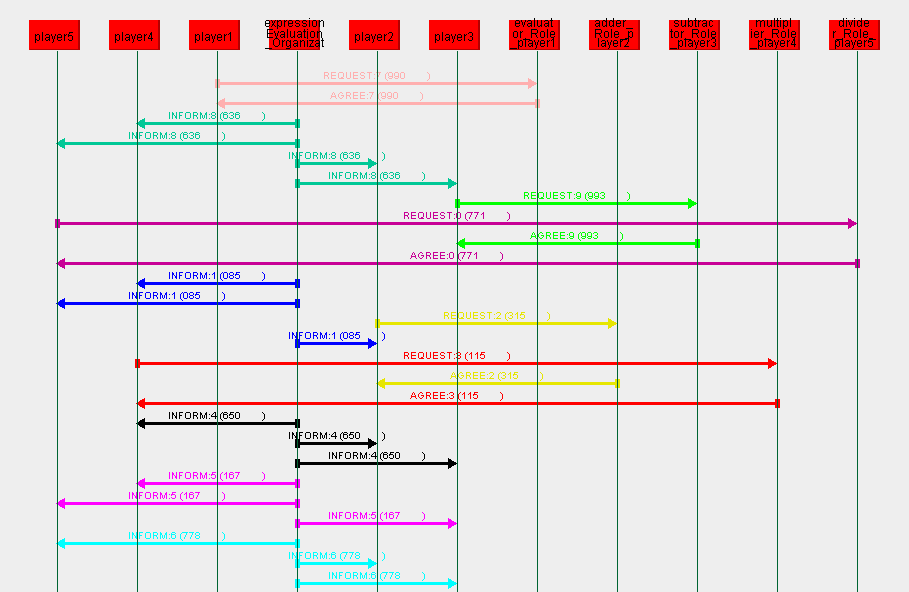
\includegraphics[width=\textwidth]{images/examples/example2-stage4.png}
	\caption{Stage 4: Role deactivation}
	\label{figure:example2-stage4}
\end{figure}

% Pink
In the {\color{pink}{\textbf{pink}}} interaction scenario, \textit{player1} deactivates its \textit{Evaluator} role.
% Teal
In the {\color{teal}{\textbf{teal}}} interaction scenario, the \textit{expression-evaluation} organization publishes the \textit{Role deactivated} event (for the \textit{Evaluator} role).
\textit{player2} reacts by deactivating its \textit{Adder} role (the {\color{yellow}{\textbf{yellow}}} interaction scenario), \textit{player3} by deactivating its \textit{Subtractor} role (the {\color{green}{\textbf{green}}} interaction scenario), \textit{player4} by deactivating its \textit{Multiplier} role (the {\color{red}{\textbf{red}}} interaction scenario) and \textit{player5} by deactivating its \textit{Divider} role (the {\color{purple}{\textbf{purple}}} interaction scenario).

% Yellow
In the {\color{yellow}{\textbf{yellow}}} interaction scenario, \textit{player2} deactivates its \textit{Adder} role.
% Magenta
In the {\color{magenta}{\textbf{magenta}}} interaction scenario, the \textit{expression-evaluation} organization publishes the \textit{Role deactivated} event (for the \textit{Adder} role).

% Green
In the {\color{green}{\textbf{green}}} interaction scenario, \textit{player3} deactivates its \textit{Subtractor} role.
% Blue
In the {\color{blue}{\textbf{blue}}} interaction scenario, the \textit{expression-evaluation} organization publishes the \textit{Role deactivated} event (for the \textit{Subtractor} role).

% Red
In the {\color{red}{\textbf{red}}} interaction scenario, \textit{player4} deactivates its \textit{Multiplier} role.
% Cyan
In the {\color{cyan}{\textbf{cyan}}} interaction scenario, the \textit{expression-evaluation} organization publishes the \textit{Role deactivated} event (for the \textit{Multiplier} role).

% Purple
In the {\color{purple}{\textbf{purple}}} interaction scenario, \textit{player5} deactivates its \textit{Divider} role.
% Black
In the {\color{black}{\textbf{black}}} interaction scenario, the \textit{expression-evaluation} organization publishes the \textit{Role deactivated} event (for the \textit{Divider} role).

%%%%%%%%%%%%%%%%%%%%%%%%%%%%%%%%%%%%%%%%%%%%%%%%%%%%%%%%%%%%%%%%%%%%%%%%%%%%%%%%
\subsubsection*{Stage 5: Role Deactment}

% Figure: Stage 5: Role deactment
\begin{figure}[H]
	\centering
	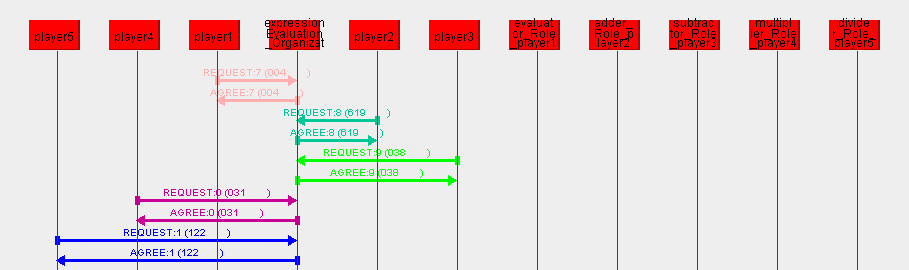
\includegraphics[width=\textwidth]{images/examples/example2-stage5.png}
	\caption{Stage 5: Role deactment}
	\label{figure:example2-stage5}
\end{figure} 

% Pink
In the {\color{pink}{\textbf{pink}}} interaction scenario, \textit{player1} deacts its \textit{Evaluator} role and the \textit{evaluator-player1} position is abolished.

% Teal
In the {\color{teal}{\textbf{teal}}} interaction scenario, \textit{player2} deacts its \textit{Adder} role and the \textit{adder-player2} position is abolished.

% Green
In the {\color{green}{\textbf{green}}} interaction scenario, \textit{player3} deacts its \textit{Subtractor} role and the \textit{subtractor-player3} position is abolished.

% Purple
In the {\color{purple}{\textbf{purple}}} interaction scenario, \textit{player4} deacts its \textit{Multiplier} role and the \textit{multiplier-player4} position is abolished.

% Blue
In the {\color{blue}{\textbf{blue}}} interaction scenario, \textit{player5} deacts its \textit{Divider} role and the \textit{divider-player5} position is abolished.

%%%%%%%%%%%%%%%%%%%%%%%%%%%%%%%%%%%%%%%%%%%%%%%%%%%%%%%%%%%%%%%%%%%%%%%%%%%%%%%%
%% Title (en): Multiagent Systems and Organizations                           %%
%% Title (cs): Multiagentní systémy a organizace                              %%
%%                                                                            %%
%% Author: Bc. Lukáš Kúdela                                                   %%
%% Supervisor: Prof. RNDr. Petr Štěpánek, DrSc.                               %%
%%                                                                            %%
%% Academic year: 2011/2012                                                   %%
%%%%%%%%%%%%%%%%%%%%%%%%%%%%%%%%%%%%%%%%%%%%%%%%%%%%%%%%%%%%%%%%%%%%%%%%%%%%%%%%

%%%%%%%%%%%%%%%%%%%%%%%%%%%%%%%%%%%%%%%%%%%%%%%%%%%%%%%%%%%%%%%%%%%%%%%%%%%%%%%%
\section{Example 3: Auction}
%%%%%%%%%%%%%%%%%%%%%%%%%%%%%%%%%%%%%%%%%%%%%%%%%%%%%%%%%%%%%%%%%%%%%%%%%%%%%%%%

% Auction organization
This example demonstrates a relatively complex organization - the auction.
% Auction organization - purpose
The purpose of this organization is to facilitate auction by bringing together several agents: one agent auctions an item and the other agents bid for it.
The item can be auctioned in an envelope, Vickrey, english or dutch auction.
% Assumptions
In this example, agents sell and buy works of art (famous paintings) in an envelope auction, but it should be obvious that any of the four auction types could be used to sell any items.

%%%%%%%%%%%%%%%%%%%%%%%%%%%%%%%%%%%%%%%%%%%%%%%%%%%%%%%%%%%%%%%%%%%%%%%%%%%%%%%%
\subsection*{Specification}

%%%%%%%%%%%%%%%%%%%%%%%%%%%%%%%%%%%%%%%%%%%%%%%%%%%%%%%%%%%%%%%%%%%%%%%%%%%%%%%%
\subsubsection*{Organization Part}

% 'Auction' organizaiton type
The \textit{Auciton} organization type (modelled by the \texttt{Auction\_Organization} agent class) contains two roles - \textit{Auctioneer} and \textit{Bider} - and four protocols - \textit{Envelope auction}, \textit{Vickrey auction}, \textit{English auction} and \textit{Dutch auction}.
% 'auction' organization
\textit{Auction} has one instance in the running MAS - the \textit{auction} organization (modelled by the \texttt{auction\_Organization} agent instance).

% 'Auctioneer' role
The \textit{Auctioneer} role (modelled by the \texttt{Auctioneer\_Role} class) can sell an item in an auction, i.e. it can auction an item.
% 'Auctioneer' role - multiplicity, competences & responsibilities
The \textit{Auctioneer} role is a \textit{single} role.
It has one competence - \textit{Auction} - and no responsibilities.

% 'Auction' competence
The \textit{Auction} competence (modelled by the \texttt{Auction\_Competence} class) is a competence to auction an item.
% 'Auction' competence - argument & result
It has several arguments depending on the type of the auction - mainly the name of the item - and several results - particularly the hammer price.

% 'Bidder' role
The \textit{Bidder} role (modelled by the \texttt{Bidder\_Role} class) can buy an item in an auction, i.e. it can bid for an item. 
% 'Bidder' role - multiplicity, competences & responsibilities
The \textit{Bidder} role is a \textit{multiple} role.
It has no competences and one responsibility - \textit{Bid}.

% 'Bid' responsibility
The \textit{Bid} responsibility (modelled by the \texttt{Bid\_Responsibility} class) is a responsibility to bid for an item.
% 'Bid' responsibility - argument & result
It has several arguments depending on the type of the auction - mainly the name of the item - and several results - the bid in particular.

%%%%%%%%%%%%%%%%%%%%%%%%%%%%%%%%%%%%%%%%%%%%%%%%%%%%%%%%%%%%%%%%%%%%%%%%%%%%%%%%
\subsubsection*{Protocol Part}

% 'Envelope acution' protocol
The \textit{Envelope auction} protocol (modelled by the \texttt{EnvelopeAuctionProtocol} class) is a protocol through which an \textit{Auctioneer} (the initiator party, modelled by the \texttt{EnvelopeAuction\_InitiatorParty} class) can determine the best buyer from among the \textit{Bidders} (responder party, modelled by the \texttt{EnvelopeAuction\_RespoderParty} class).
% Envelope auction
The Envelope auction is a sealed bid first-price auction.
In this type of auction the sealed bids (unknown to other bidders) are submitted simultaneously to the auctioneer and the item is sold to the winning bidder for the price of their bid.

% Vickrey auction protocol
The \textit{Vickrey auction} protocol (modelled by the \texttt{VickreyAuctionProtocol} class) is a protocol through which an \textit{Auctioneer} (the initiator party, modelled by the \texttt{VickreyAuction\_InitiatorParty} class) can choose the best buyer from among the \textit{Bidders} (responder party, modelled by the \texttt{VickreyAuction\_RespoderParty} class).
% Vickrey auction
The Vickrey auction is a sealed bid second-price auction.
In this type of auction the sealed bids are submitted simultaneously to the auctioneer and the item is sold to the winning bidder for the price of the \textit{second} highest bid.

% English auction protocol
The \textit{English auction} protocol (modelled by the \texttt{EnglishAuctionProtocol} class) is a protocol through which an \textit{Auctioneer} (the initiator party, modelled by the \texttt{EnglishAuction\_InitiatorParty} class) can determine the best buyer from among the \textit{Bidders} (responder party, modelled by the \texttt{EnglishAuction\_RespoderParty} class).
% English auction
The English auction is an open bid ascending price auction.
In this type of auction the auctioneer announces the starting price (lower than the expected selling price).
The bidders then sequentially submit open bids in ascending fashion, respecting the minimum increment.
The item is sold to the \textit{last} bidder willing to pay the price.

% Dutch auction protocol
The \textit{Dutch auction} protocol (modelled by the \texttt{DutchAuctionProtocol} class) is a protocol through which an \textit{Auctioneer} (the initiator party, modelled by the \texttt{DutchAuction\_InitiatorParty} class) can determine the best buyer from among the \textit{Bidders} (responder party, modelled by the \texttt{DutchAuction\_RespoderParty} class).
% Dutch auction
The Dutch auction is an open bid descending price auction.
In this type of auction the auctioneer announces a starting price (higher than the expected selling price).
The auctioneer then sequentially offers prices in descending fashion, respecting the minimum decrement.
The item is sold to the \textit{first} bidder willing to pay the price.

% 'Auction call-for-proposals' message
The \textit{Auction call-for-proposals (CFP)} message (modelled by the \texttt{AuctionCFPMessage} class) is a message sent by an \textit{Auctioneer} to all \textit{Bidders} calling for proposals for the auctioned item's price.

% 'Bid propose' message
The \textit{Bid propose} message (modelled by the \texttt{BidProposeMessage} class) is a message sent by a \textit{Bidder} to an \textit{Auctioneer} proposing a bid to the latter.

%%%%%%%%%%%%%%%%%%%%%%%%%%%%%%%%%%%%%%%%%%%%%%%%%%%%%%%%%%%%%%%%%%%%%%%%%%%%%%%%
\subsubsection*{Player Part}

% 'Participant' player type
The \textit{Participant} player type (modelled by the \texttt{Participant} agent class) is a player capable of biding for an item.
\textit{Participant} has three instances in the running MAS - \textit{player1}, \textit{player2} and \textit{player3}.
All of them intend to enact both the \textit{Auctioneer} and \textit{Bidder} roles in the \textit{auction} organization and perform the \textit{Auctioneer} role's \textit{Auction} competence - to auction an item to the players of the \textbf{Bidder} role.
They also intend to perform the \textit{Bidder} role's \textit{Bid} responsibility - to bid for an item auctioned by the player of the \textit{Auctioneer} role.
% 'player1' player
\textit{player1} (modelled by the \texttt{player1} agent instance) intends to play the \textbf{Auctioneer} in the first round and be the \textbf{Bidder} in the second and third rounds.
% 'player2' player
\textit{player2} (modelled by the \texttt{player2} agent instance) intends to be the \textit{Auctioneer} in the second round and play the \textit{Bidder} in the first and third rounds.
% 'player3' player
\textit{player3} (modelled by the \texttt{player3} agent instance) intends to play the \textit{Auctioneer} in the third rounds and be the \textit{Bidder} in the first and second rounds.

%%%%%%%%%%%%%%%%%%%%%%%%%%%%%%%%%%%%%%%%%%%%%%%%%%%%%%%%%%%%%%%%%%%%%%%%%%%%%%%%
\section{Manifestation} 

%%%%%%%%%%%%%%%%%%%%%%%%%%%%%%%%%%%%%%%%%%%%%%%%%%%%%%%%%%%%%%%%%%%%%%%%%%%%%%%%
\subsubsection*{Stage 3: Competence and Responsibility Invocation}

% Figure: Stage 3: Competence and responsibility invocation
\begin{figure}[H]
	\centering
	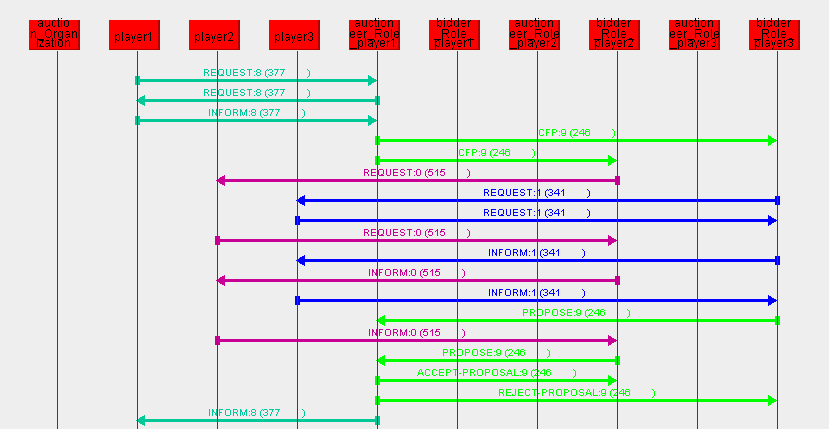
\includegraphics[width=\textwidth]{images/examples/example3-stageA3.png}
	\caption{Stage 3: Competence and responsibility invocation}
	\label{figure:example3-stageA3}
\end{figure}

First, \textit{player1} invokes the \textit{Auction} competence from its \textit{auctioneer-player1} position with parameters of the auction - the name of the item and the reservation price (the \textbf{dark green} interaction scenario).
\textit{auctioneer-player1} calls for proposals for the item price from all \textit{Bidder} positions (the \textbf{light green} interaction scenario).
To come up with their bids, the \textit{bidder-player2} and \textit{bidder-player3} invoke the \textit{Bid} responsibilities from \textit{player2} and \textit{player3} respectively (the \textbf{purple} and \textbf{blue} interaction scenarios respectively).
\textit{bidder-player2} and \textit{bidder-player3} propose their bids to \textit{auctioneer-player1} who determines if the auction is successful or not, i. e. whether the auction winner has been found.
If the highest bid is at least as high as the reservation price, the auction is successful, the winner is the highest bidding bidder and the hammer price is their bid; otherwise, the auction is unsuccessful.
Next, \textit{auctioneer-player1} informs the winner (if there is one) that his proposal has been accepted and all other bidders that their proposal has been rejected.
Finally, \textit{auctioneer-player1} informs \textit{player1} about the outcome of the auction - whether it was successful or not and in case it were, who is the winner and what is the hammer price (the \textbf{dark green} interaction scenario again).